

\tikzset{every picture/.style={line width=0.75pt}} %set default line width to 0.75pt        

\begin{tikzpicture}[x=0.75pt,y=0.75pt,yscale=-1,xscale=1]
	\fontsize{11pt}{12pt}\selectfont
	%uncomment if require: \path (0,217); %set diagram left start at 0, and has height of 217
	
	%Image [id:dp6889538666297523] 
	\draw (259,106.73) node  {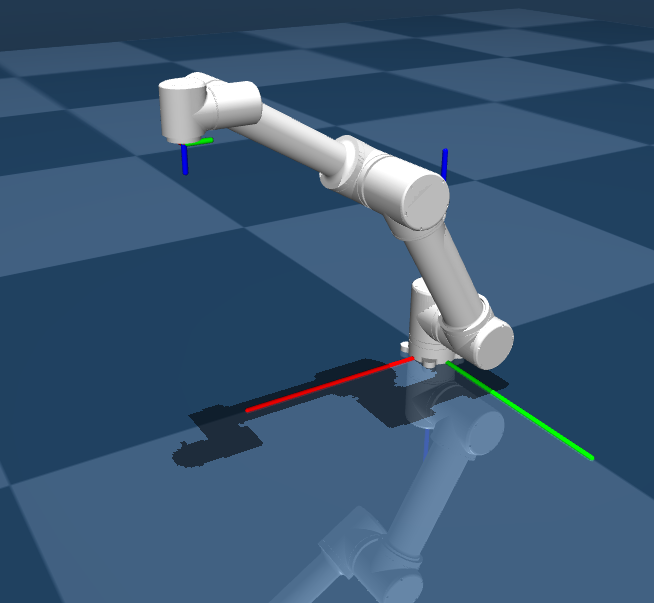
\includegraphics[width=159pt,height=146.6pt]{robot7dof.png}};
	%Curve Lines [id:da580161720299337] 
	\draw [color={rgb, 255:red, 0; green, 255; blue, 0 }  ,draw opacity=1 ]   (215,66.54) .. controls (235,121.54) and (235,180.54) .. (391,173.54) ;
	\draw [shift={(391,173.54)}, rotate = 177.43] [color={rgb, 255:red, 0; green, 255; blue, 0 }  ,draw opacity=1 ][line width=0.75]    (10.93,-3.29) .. controls (6.95,-1.4) and (3.31,-0.3) .. (0,0) .. controls (3.31,0.3) and (6.95,1.4) .. (10.93,3.29)   ;
	%Curve Lines [id:da09242711224450773] 
	\draw [color={rgb, 255:red, 0; green, 255; blue, 0 }  ,draw opacity=1 ]   (593,177.54) .. controls (640.52,157.74) and (634.13,88.94) .. (593.25,65.25) ;
	\draw [shift={(592,64.54)}, rotate = 28.71] [color={rgb, 255:red, 0; green, 255; blue, 0 }  ,draw opacity=1 ][line width=0.75]    (10.93,-3.29) .. controls (6.95,-1.4) and (3.31,-0.3) .. (0,0) .. controls (3.31,0.3) and (6.95,1.4) .. (10.93,3.29)   ;
	%Curve Lines [id:da6843282504138404] 
	\draw [color={rgb, 255:red, 0; green, 255; blue, 0 }  ,draw opacity=1 ]   (464,54.54) .. controls (429.35,28.8) and (278.07,23.64) .. (234.29,37.13) ;
	\draw [shift={(233,37.54)}, rotate = 341.57] [color={rgb, 255:red, 0; green, 255; blue, 0 }  ,draw opacity=1 ][line width=0.75]    (10.93,-3.29) .. controls (6.95,-1.4) and (3.31,-0.3) .. (0,0) .. controls (3.31,0.3) and (6.95,1.4) .. (10.93,3.29)   ;
	%Curve Lines [id:da8394696818177255] 
	\draw [color={rgb, 255:red, 0; green, 255; blue, 0 }  ,draw opacity=1 ]   (449,57.54) .. controls (389.6,44.67) and (320.4,42.58) .. (274.39,59.04) ;
	\draw [shift={(273,59.54)}, rotate = 339.72] [color={rgb, 255:red, 0; green, 255; blue, 0 }  ,draw opacity=1 ][line width=0.75]    (10.93,-3.29) .. controls (6.95,-1.4) and (3.31,-0.3) .. (0,0) .. controls (3.31,0.3) and (6.95,1.4) .. (10.93,3.29)   ;
	%Curve Lines [id:da09158135447808469] 
	\draw [color={rgb, 255:red, 0; green, 255; blue, 0 }  ,draw opacity=1 ]   (451,71.54) .. controls (391.6,89.36) and (353.76,97.38) .. (294.79,80.07) ;
	\draw [shift={(293,79.54)}, rotate = 16.7] [color={rgb, 255:red, 0; green, 255; blue, 0 }  ,draw opacity=1 ][line width=0.75]    (10.93,-3.29) .. controls (6.95,-1.4) and (3.31,-0.3) .. (0,0) .. controls (3.31,0.3) and (6.95,1.4) .. (10.93,3.29)   ;
	%Curve Lines [id:da5298341943704198] 
	\draw [color={rgb, 255:red, 0; green, 255; blue, 0 }  ,draw opacity=1 ]   (458,81.54) .. controls (421.18,116.37) and (379.42,131.39) .. (313.99,119.72) ;
	\draw [shift={(313,119.54)}, rotate = 10.3] [color={rgb, 255:red, 0; green, 255; blue, 0 }  ,draw opacity=1 ][line width=0.75]    (10.93,-3.29) .. controls (6.95,-1.4) and (3.31,-0.3) .. (0,0) .. controls (3.31,0.3) and (6.95,1.4) .. (10.93,3.29)   ;
	%Curve Lines [id:da9873811746998208] 
	\draw [color={rgb, 255:red, 208; green, 2; blue, 27 }  ,draw opacity=1 ] [dash pattern={on 4.5pt off 4.5pt}]  (295,121.54) .. controls (256.39,190.84) and (178.58,191.53) .. (134.33,170.2) ;
	\draw [shift={(133,169.54)}, rotate = 26.57] [color={rgb, 255:red, 208; green, 2; blue, 27 }  ,draw opacity=1 ][line width=0.75]    (10.93,-3.29) .. controls (6.95,-1.4) and (3.31,-0.3) .. (0,0) .. controls (3.31,0.3) and (6.95,1.4) .. (10.93,3.29)   ;
	%Curve Lines [id:da7589617847853484] 
	\draw [color={rgb, 255:red, 208; green, 2; blue, 27 }  ,draw opacity=1 ] [dash pattern={on 4.5pt off 4.5pt}]  (275,69.54) .. controls (236.58,138.49) and (183.62,135.65) .. (140.94,141.28) ;
	\draw [shift={(139,141.54)}, rotate = 352.06] [color={rgb, 255:red, 208; green, 2; blue, 27 }  ,draw opacity=1 ][line width=0.75]    (10.93,-3.29) .. controls (6.95,-1.4) and (3.31,-0.3) .. (0,0) .. controls (3.31,0.3) and (6.95,1.4) .. (10.93,3.29)   ;
	%Curve Lines [id:da25165735151019264] 
	\draw [color={rgb, 255:red, 208; green, 2; blue, 27 }  ,draw opacity=1 ] [dash pattern={on 4.5pt off 4.5pt}]  (232,44.54) .. controls (248.75,104.63) and (185.93,122.99) .. (142.95,129.26) ;
	\draw [shift={(141,129.54)}, rotate = 352.06] [color={rgb, 255:red, 208; green, 2; blue, 27 }  ,draw opacity=1 ][line width=0.75]    (10.93,-3.29) .. controls (6.95,-1.4) and (3.31,-0.3) .. (0,0) .. controls (3.31,0.3) and (6.95,1.4) .. (10.93,3.29)   ;
	%Curve Lines [id:da5507245481753484] 
	\draw [color={rgb, 255:red, 208; green, 2; blue, 27 }  ,draw opacity=1 ] [dash pattern={on 4.5pt off 4.5pt}]  (84,125.54) .. controls (72.18,112.74) and (76.85,118.37) .. (75.09,81.27) ;
	\draw [shift={(75,79.54)}, rotate = 87.06] [color={rgb, 255:red, 208; green, 2; blue, 27 }  ,draw opacity=1 ][line width=0.75]    (10.93,-3.29) .. controls (6.95,-1.4) and (3.31,-0.3) .. (0,0) .. controls (3.31,0.3) and (6.95,1.4) .. (10.93,3.29)   ;
	%Curve Lines [id:da6098588780506541] 
	\draw [color={rgb, 255:red, 208; green, 2; blue, 27 }  ,draw opacity=1 ] [dash pattern={on 4.5pt off 4.5pt}]  (215,66.54) .. controls (203.24,53.8) and (118.49,42.02) .. (89.69,50.97) ;
	\draw [shift={(88,51.54)}, rotate = 339.68] [color={rgb, 255:red, 208; green, 2; blue, 27 }  ,draw opacity=1 ][line width=0.75]    (10.93,-3.29) .. controls (6.95,-1.4) and (3.31,-0.3) .. (0,0) .. controls (3.31,0.3) and (6.95,1.4) .. (10.93,3.29)   ;
	
	% Text Node
	\draw (396,160) node [anchor=north west][inner sep=0.75pt]   [align=left] {framepos and framequad for \\getting end-effector pose};
	% Text Node
	\draw (465,58.54) node [anchor=north west][inner sep=0.75pt]   [align=left] {hinge joints values};
	% Text Node
	\draw (498,112.33) node [anchor=north west][inner sep=0.75pt]   [align=left] {inverse kinematics};
	% Text Node
	\draw (70,126) node [anchor=north west][inner sep=0.75pt]   [align=left] {forward \\kinematics};
	% Text Node
	\draw (60,53) node [anchor=north west][inner sep=0.75pt]   [align=left] {comparation};
	
	
\end{tikzpicture}